\subsection{方法二：排除最优路线后的搜索}

示例程序搜索的是概率最高的单条四轮差分路线。设 $\Delta_0$ 为输入差分，$\Delta_r$ 为第 $r$ 轮经过 S 盒和 P 置换后的差分，则一条路线写为
\[
    \Delta_0\rightarrow\Delta_1\rightarrow\Delta_2
    \rightarrow\Delta_3\rightarrow\Delta_4.
\]
程序得到的最优路线为
\[
    \text{0x}0001\rightarrow\text{0x}0001
    \rightarrow\text{0x}0001\rightarrow\text{0x}0001
    \rightarrow\text{0x}0001,
\]
每轮传播概率均为 $1/2$，所以该路线的概率为 $(1/2)^4=1/16$。为了判断是否存在概率相同的其他路线，需要在搜索中排除这条已知路线。

\subsubsection{排除路线的依据}

设 $B_r(\Delta)$ 表示经过 $r$ 轮后到达差分状态 $\Delta$ 的最大单条路线概率。一轮差分转移概率仍记为 $R(u,v)$，则示例程序的更新规则可写为
\[
    B_{r+1}(v)=\max_u\bigl\{B_r(u)R(u,v)\bigr\}.
\]
这里取最大值，与方法一中对所有前驱路线求和不同。初始化时，所有非零输入差分的 $B_0$ 均设为 $1$，而 $B_0(0)=0$。这是因为零输入差分会以概率 $1$ 沿全零路线传播；将其排除，才能搜索非零差分路线。

原最优路线在 $\Delta_0,\ldots,\Delta_4$ 的五个位置上均为 $\text{0x}0001$。任意另一条路线至少有一个位置与之不同，因此可以分别在位置 $j=0,1,2,3,4$ 禁用差分 $\text{0x}0001$，对五次搜索结果取最大概率。五个受限搜索覆盖了所有不同于原最优路线的路线；某条路线若在多个位置不同，也可能在多次搜索中重复出现。

实现时，$j=0$ 对应将初始概率数组的 $\text{0x}0001$ 项置零；$j=1,\ldots,4$ 对应在第 $j$ 轮完成 S 盒和 P 置换后，将 $B_j(\text{0x}0001)$ 置零。每次四轮搜索结束后，再由最终状态逆向追溯各轮差分，得到完整路线。图~\ref{fig:task1_method2_code} 展示了代码中的位置参数和禁用操作。

\begin{figure}[H]
    \centering
    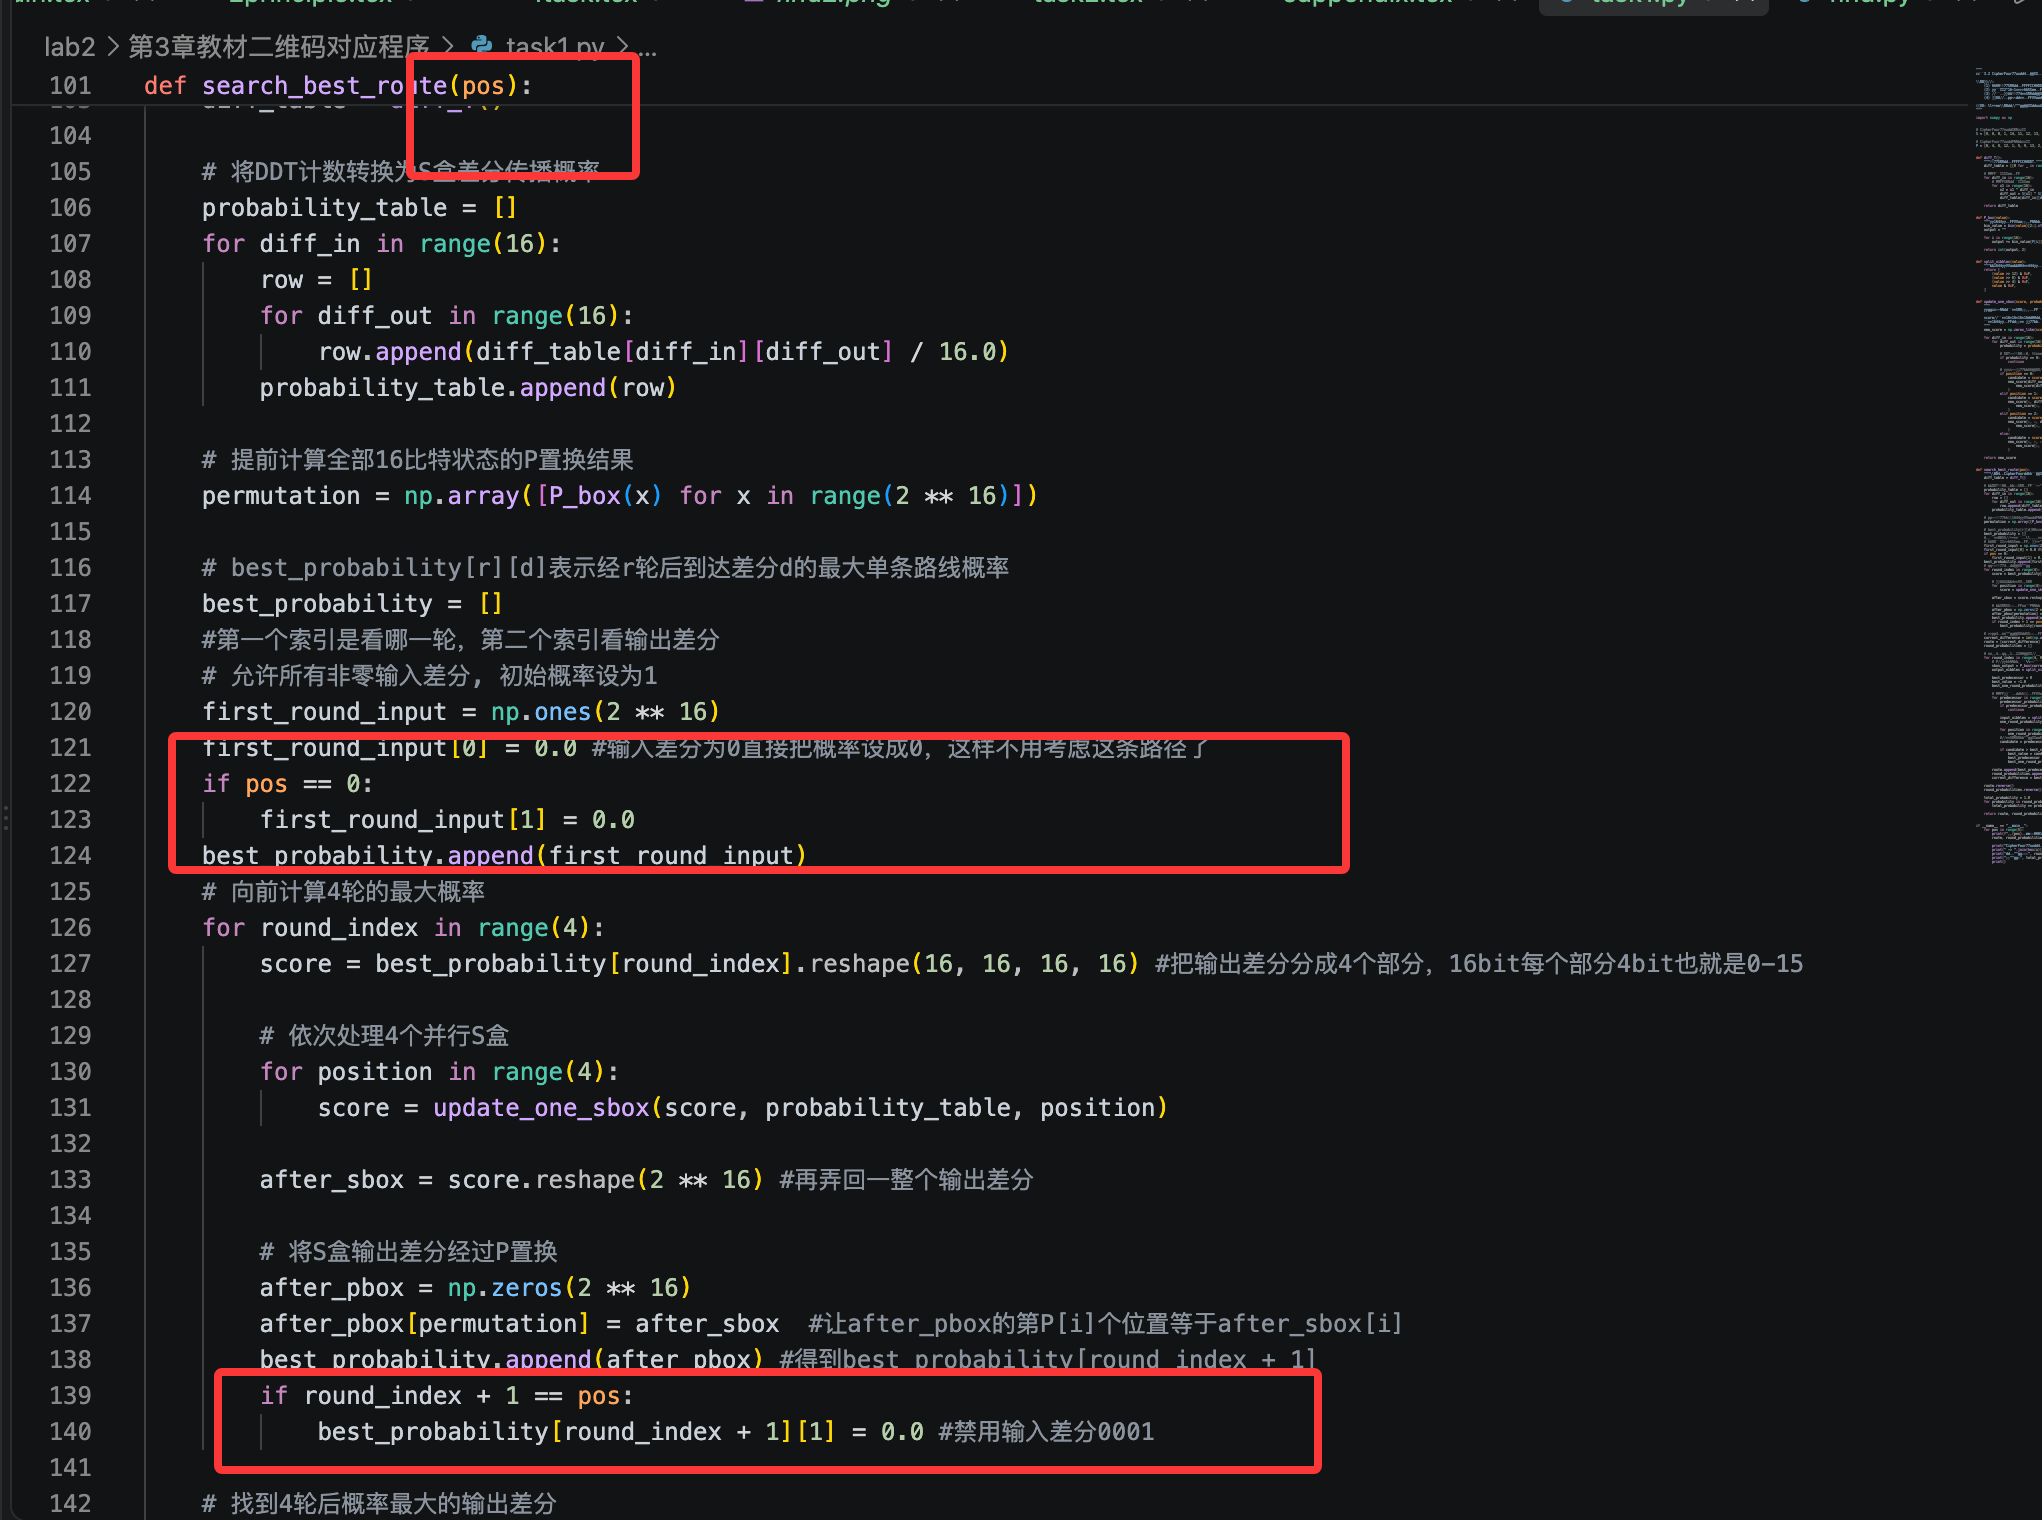
\includegraphics[width=0.8\textwidth]{figures/task1_enhance.png}
    \caption{在指定位置排除已知最优路线的差分状态}
    \label{fig:task1_method2_code}
\end{figure}

\subsubsection{搜索结果}

图~\ref{fig:task1_method2_result} 给出五次受限搜索的输出。表~\ref{tab:task1_method2_result} 将各路线整理为十六进制差分状态序列，并按四轮概率的乘积给出路线概率。

\begin{figure}[H]
    \centering
    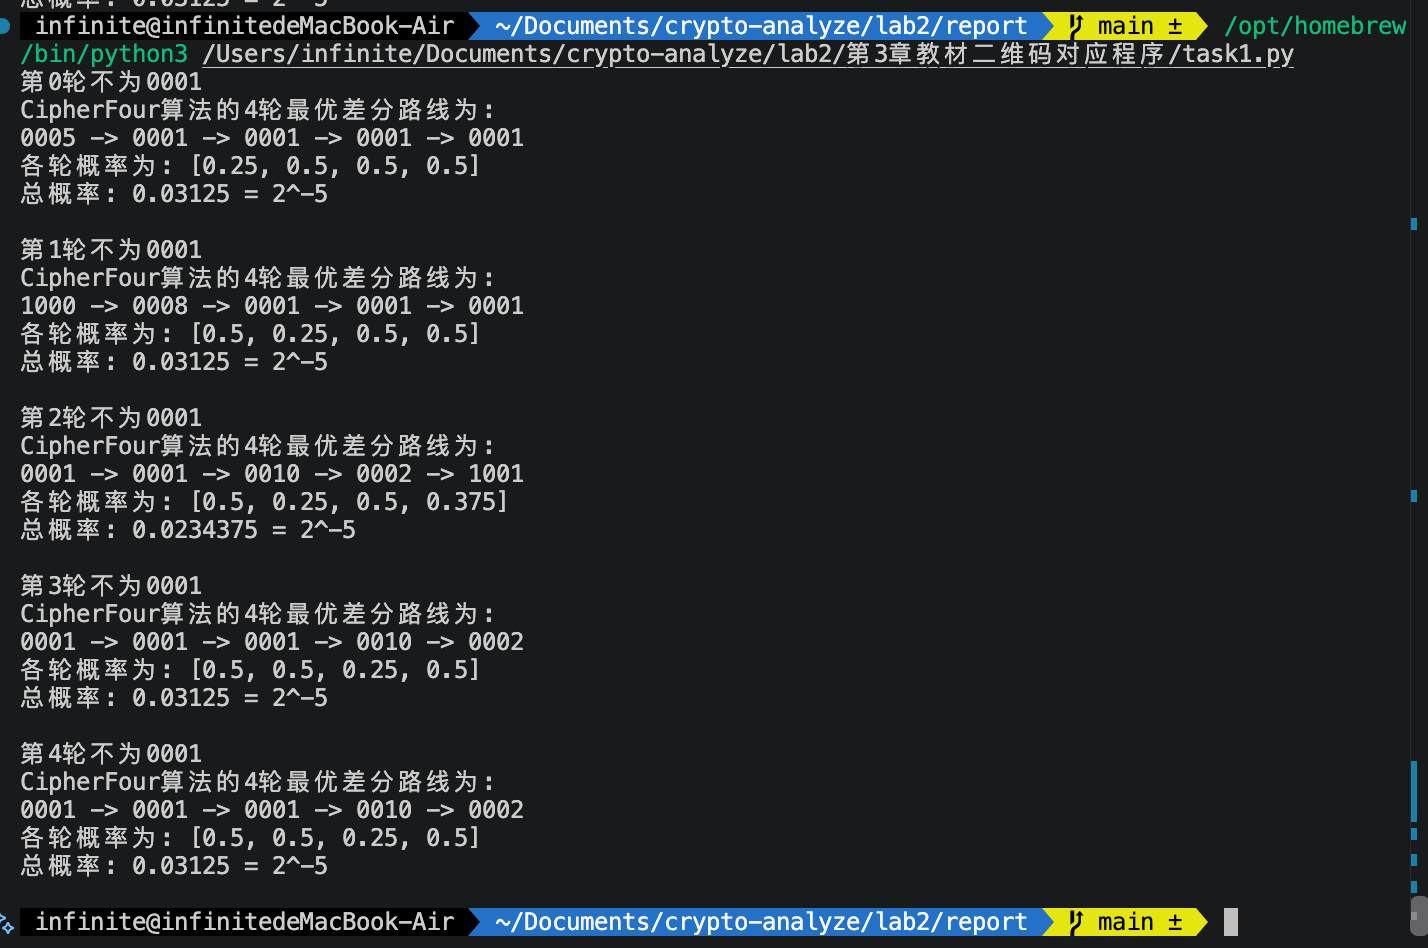
\includegraphics[width=0.8\textwidth]{figures/task1_result.png}
    \caption{分别禁用五个位置后的差分路线搜索结果}
    \label{fig:task1_method2_result}
\end{figure}

\begin{table}[H]
    \centering
    \small
    \caption{排除已知最优路线后得到的差分路线}
    \label{tab:task1_method2_result}
    \renewcommand{\arraystretch}{1.15}
    \begin{tabular}{ccl}
        \toprule
        禁用位置 $j$ & 路线概率 & 差分路线（十六进制） \\
        \midrule
        0 & $1/32$ & $0005\to0001\to0001\to0001\to0001$ \\
        1 & $1/32$ & $1000\to0008\to0001\to0001\to0001$ \\
        2 & $3/128$ & $0001\to0001\to0010\to0002\to1001$ \\
        3 & $1/32$ & $0001\to0001\to0001\to0010\to0002$ \\
        4 & $1/32$ & $0001\to0001\to0001\to0010\to0002$ \\
        \bottomrule
    \end{tabular}
\end{table}

在禁用位置 $j=2$ 的一次搜索中，四轮概率分别为 $1/2,1/4,1/2,3/8$，实际乘积为 $3/128=0.0234375$。截图末尾的 $2^{-5}$ 是程序对概率取对数后再转为整数的显示结果，不能作为这条路线的精确概率。其余四次受限搜索均得到 $1/32$。因此，排除原最优路线后，概率最高的单条路线为 $1/32$，低于原路线的 $1/16$；位置 $j=3$ 与 $j=4$ 搜索到了同一条路线，五次结果共对应四条不同路线。

这些结果反映的是单条差分路线的概率。若只看输入、输出差分，上述四条路线分别对应 $\text{0x}0005\to\text{0x}0001$、$\text{0x}1000\to\text{0x}0001$、$\text{0x}0001\to\text{0x}1001$ 和 $\text{0x}0001\to\text{0x}0002$。同一输入、输出差分还可能由其他路线实现，因此这些路线概率不能直接当作对应差分的总概率；差分总概率应按方法一对所有路线求和。
